\rhead{Object Seeking}


\chapter{Object Seeking}
\label{sec:object_seeking}

\begin{figure}[!h]
\centering
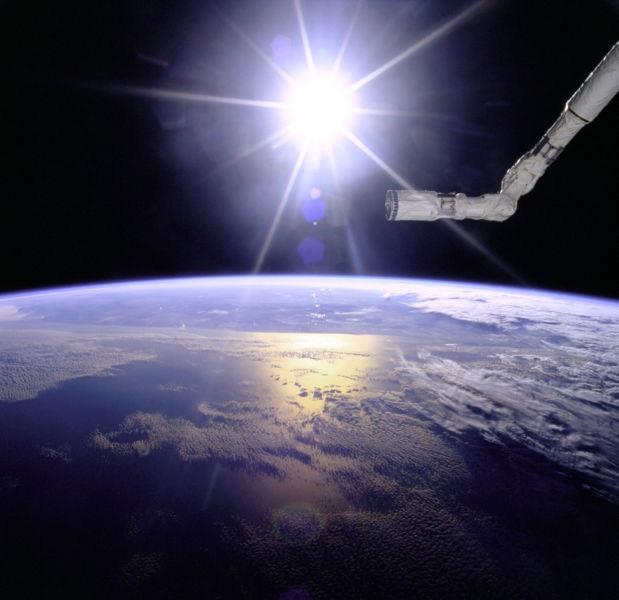
\includegraphics[width=0.9\columnwidth]{figures/6_619px-Robot_Arm_Over_Earth_with_Sunburst.jpg}
\end{figure}

\newpage

\section{Introduction}

In the Enclosure Escape assignment detailed in Chapter \ref{sec:enclosure_escape}, students were introduced to either the 
Player/Stage/Gazebo (PSG) or ROS robot interface.  The previous assignment demonstrated how to interact with real SmURV robots using 
one of these two middleware systems.  Students should now be familiar with reading sensor data and sending control commands via teleoperation 
and a client program. 

In this assignment, students will be extending your control client to perform an object seeking task.  In this seeking task, your robot will 
look for and drive to objects (``fiducials'' or ``landmarks'') that are recognizable from visual sensing (i.e., camera).  For this 
assignment, you will be working with the SmURV platform and a USB webcam.  The Player camera proxy provides 
direct access to the camera image and various parameters.  However, you should used the Player blobfinder proxy, which performs color 
segmentation and provides a set of bounding boxes around approximately solid color image regions.  While laser rangefinders provide more 
accurate information, cameras are often more practical in terms of their cost, weight, size, and sampling frequency.  Cameras have the 
additional benefit of sensing color, which you will leverage in this assignment. 

Given a world with a set of salient objects, your goal for this assignment is to create a client that continually drives between 
these objects.  Your controller's decision making should be a finite state machine (FSM).  This FSM should use one bit of state to specify 
the currently sought fiducial.  For motion control, you should use proportional-derivative (PD) servoing to center objects in the robot's 
field of view.  As a whole, your controller should put the current object in the center of view, drive as close as possible to an object 
without hitting it, flip the state bit, and continue the process for the next fiducial.

For object recognition, you will use the blobfinder proxy in Player.  The blobfinder proxy examines the images from the camera and groups 
like-colored pixels of a particular color into regions, or ``blobs.''  The blobfinder proxy returns information about detected blobs and 
their bounding boxes in the image.  The specification for the 
\href{http://playerstage.sourceforge.net/doc/Player-2.0.0/player/group\_\_playerc\_\_proxy\_\_blobfinder.html}{blobfinder proxy} can be 
found from the Player manual 
online\footnote{http://playerstage.sourceforge.net/doc/Player-2.0.0/player/classPlayerCc\_1\_1BlobfinderProxy.html\#c70f6fd71e7b47b5a5fc11e752abf75f}.

\vspace{5 mm}

\noindent At the end of this chapter you will be able to...

\begin{itemize}
\item Implement a control policy to continually seek and visit a particular set of objects in sequence.
\end{itemize}

\section{Key Concepts}

\noindent This project addresses new approaches to Perception, Decision Making and Motion Control, as seen in Figure \ref{fig:6_control_loop}), which is a part of the Robot Control Loop presented in Figure \ref{fig:1_control_loop}. To be able to recognize objects in the robot's visual stream, visual color sensing and blobfinding are employed for Perception. To continually seek and drive to a set of objects in sequence, a finite state machine is used to handle Decision Making. Finally a proprotional-derivative controller is implemented as the Motion Control, enabling the robot to actually drive to a given object in sight.

\begin{figure}[!h]
\centering
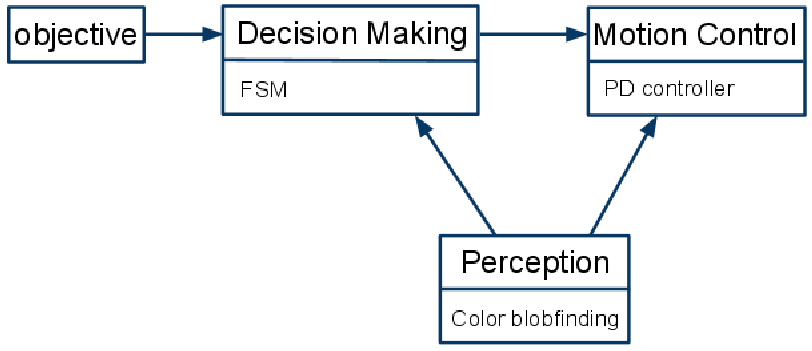
\includegraphics[width=0.5\textwidth]{figures/6_control_loop.png}
\caption{Approaches to the Object Seeking task cast within the Robot Control Loop.}
\label{fig:6_control_loop}
\end{figure}

\subsection{Color Blobfinding for Object Recognition}

\begin{figure}[!h]
\centering
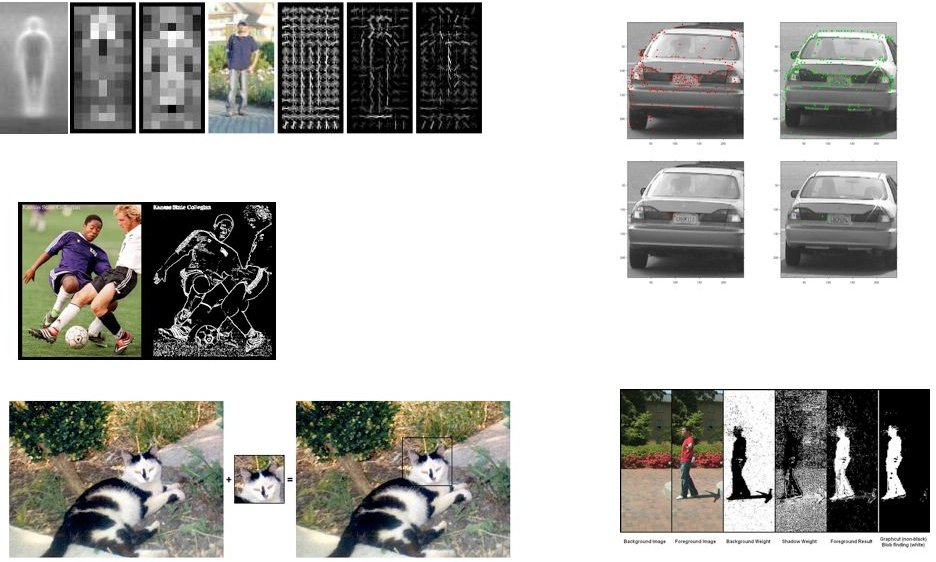
\includegraphics[width=0.8\textwidth]{figures/6_features.jpg}
\caption{Different approaches to detecting appearance features}
\end{figure}

1. object recognition
\begin{itemize}
\item training: build database of object appearance\\
- collect representative images of objects\\
- store and extract features from these images\\
- features describe object appearance\\
\item given a new image: search over image for object\\
- find database entries with features matching those in the image
\end{itemize}

2. blobfinder\\
video4l2. camerauvc; blobfinder\\

\begin{figure}[!h]
\centering
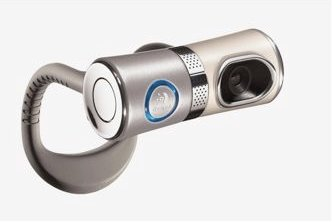
\includegraphics[width=0.4\textwidth]{figures/6_webcam.jpg}
\end{figure}

\begin{figure}[!h]
\centering
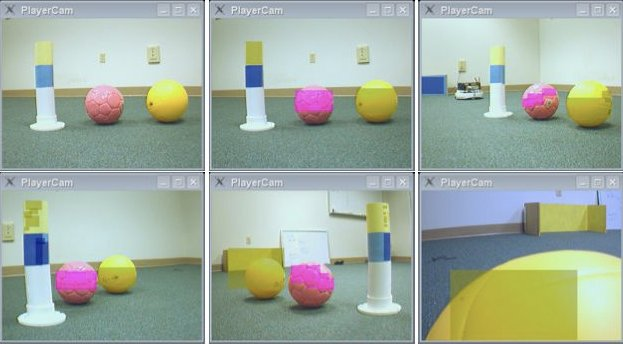
\includegraphics[width=0.9\textwidth]{figures/6_playercam.jpg}
\end{figure}

3. color blobfinding\\
input image; color threshold using color calibration; group regions based on connected components\\

\begin{figure}[!h]
\centering
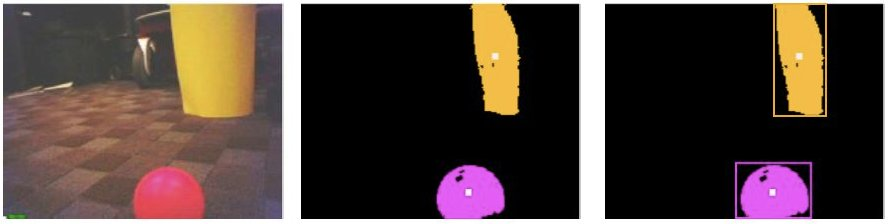
\includegraphics[width=0.9\textwidth]{figures/6_blobfinding.jpg}
\footnote{\bkorel{cite Grollman}}
\end{figure}

4. color calibration\\
blobcolors.txt example (thresholds in YUV color space)\\
playercam\_yuv output:\\

\begin{figure}[!h]
\centering
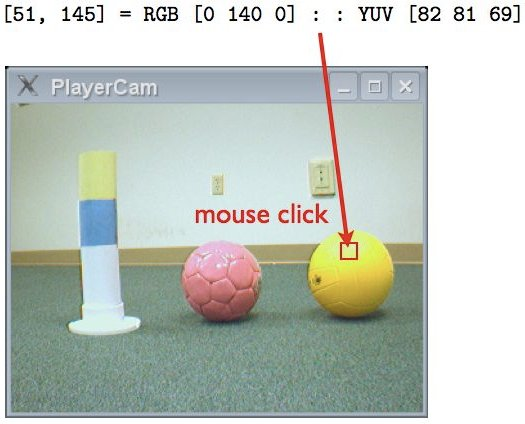
\includegraphics[width=0.5\textwidth]{figures/6_color_calibration.jpg}
\end{figure}

\subsection{Finite State Machine}

\begin{figure}[!h]
\centering
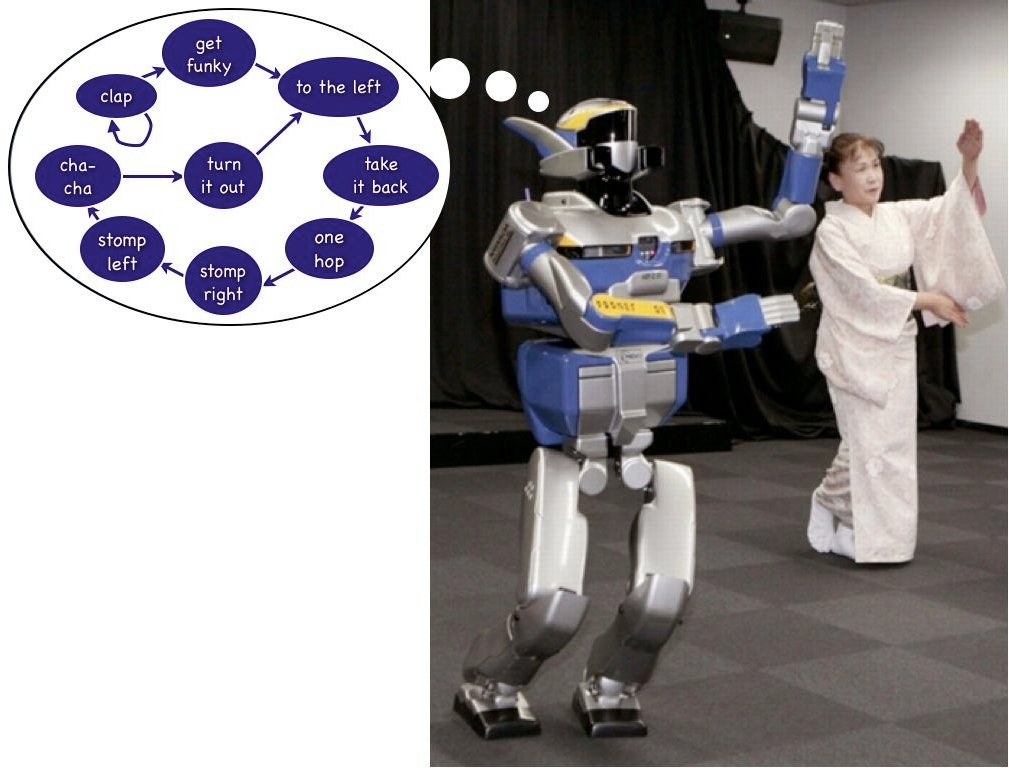
\includegraphics[width=0.6\textwidth]{figures/6_fsm_chacha.jpg}
\end{figure}

\begin{itemize}
\item components
\begin{itemize}
\item alphabet (or inputs); ``observations" in robotics
\item states
\item transitions (between states)
\end{itemize}
\end{itemize}

\begin{figure}[!h]
\centering
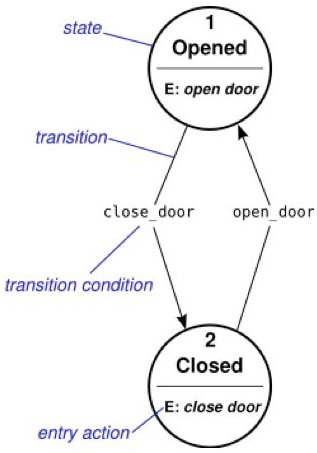
\includegraphics[width=50mm]{figures/6_general_fsm.jpg}
\footnote{\bkorel{cite wikipedia?}}
\end{figure}

Recognize the string ``nice"\\
Robotics use: preconditions (enter state) and postconditions (exit state)\\

\begin{figure}[!h]
\centering
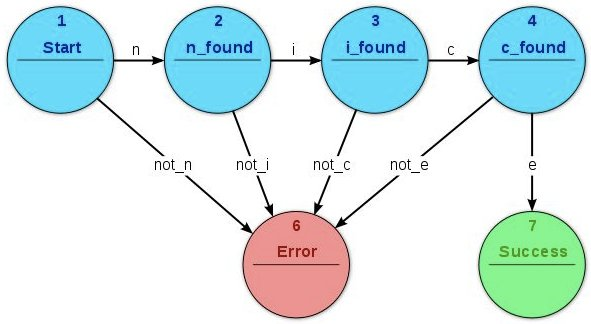
\includegraphics[width=0.65\textwidth]{figures/6_nice_fsm.jpg}
\end{figure}

Move to objects in sequence?\\
\begin{itemize}
\item How can our robot move to a given sequence of objects?\\
-yellow ball\\
-green/orange landmark\\
-pink landmark\\
-orange/green landmark\\
\item what are the states?
\item what are the transitions?
\item preconditions for states?
\item postconditions for states?
\end{itemize}

\begin{figure}[!h]
\centerline{
\mbox{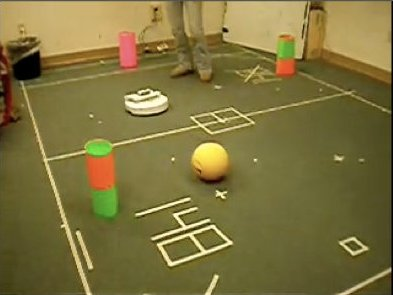
\includegraphics[height=2.0in,width=2.5in]{figures/6_move_to_objs1.jpg}}
\mbox{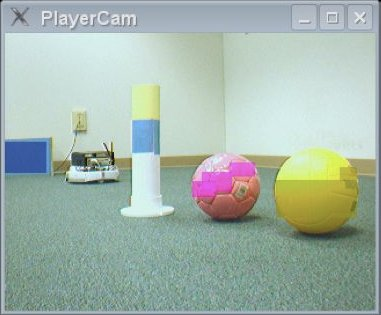
\includegraphics[height=2.0in,width=2.5in]{figures/6_move_to_objs2.jpg}}
}
\end{figure}

Object seeking FSM\\

\begin{figure}[!h]
\centering
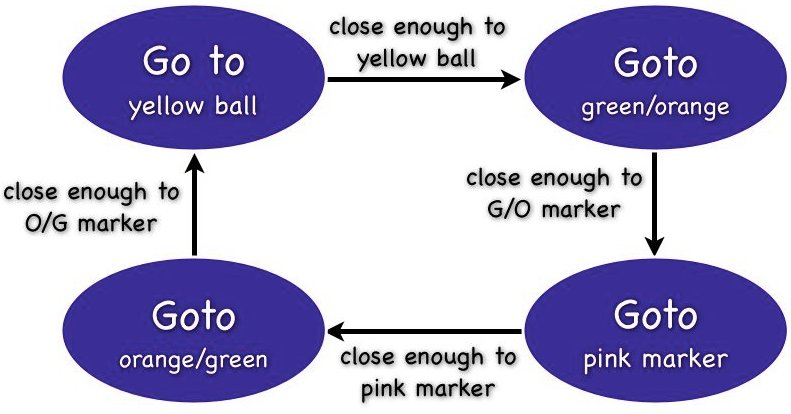
\includegraphics[width=0.65\textwidth]{figures/6_robot_fsm.jpg}
\end{figure}

\begin{figure}
\centerline{
\mbox{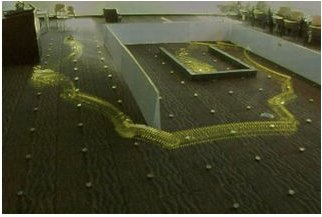
\includegraphics[width=2.10in]{figures/6_fsm_task1.jpg}}
\mbox{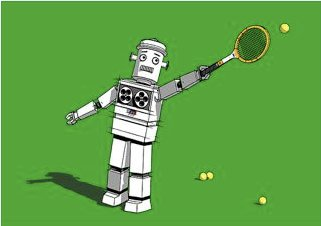
\includegraphics[width=2.015in]{figures/6_fsm_task2.jpg}}
\mbox{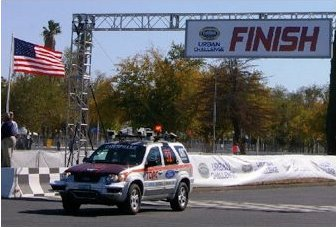
\includegraphics[width=2.10in]{figures/6_fsm_task3.jpg}}
}
\caption{FSMs for Other Tasks}
\end{figure}


\subsection{Feedback Control}

\subsubsection{Control Theory}

\begin{itemize}
\item control theory: study of behavior of dynamical systems
\item forms of control systems:
\begin{itemize}
\item open-loop control: without system feedback
\item close-loop control: adjusts to sensor observations\\
- feedback control: minimize sensed error
\item open and closed loop\\
- feedback-feedforward: predict and correct
\end{itemize}
\item important properties: stability, robustness, controllability
\end{itemize}

\begin{figure}[!h]
\centering
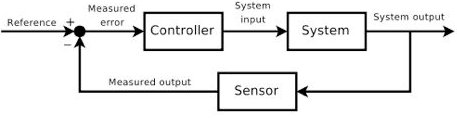
\includegraphics[width=0.65\textwidth]{figures/6_control_theory.jpg}
\end{figure}

\subsubsection{How to Move to the Ball?}

\begin{figure}[!h]
\centerline{
\mbox{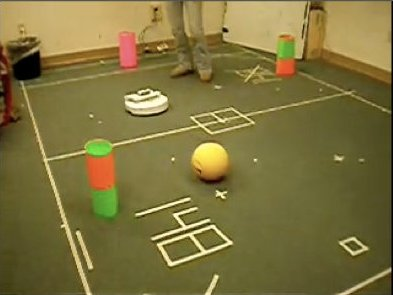
\includegraphics[height=2.0in,width=2.5in]{figures/6_move_to_objs1.jpg}}
\mbox{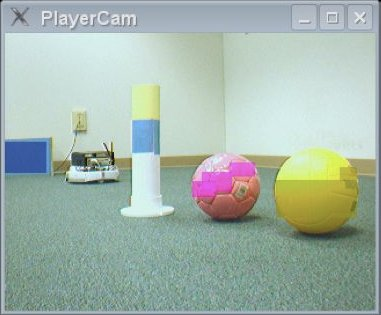
\includegraphics[height=2.0in,width=2.5in]{figures/6_move_to_objs2.jpg}}
}
\end{figure}

\begin{itemize}
\item One approach
\begin{itemize}
\item center ball in image
\item once centered, drive forward
\item can we state in terms of vx and va?
\end{itemize}

\begin{figure}[!h]
\centering
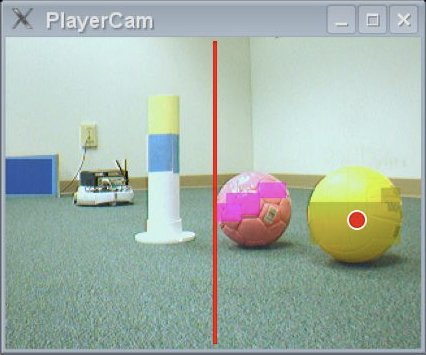
\includegraphics[width=0.5\textwidth]{figures/6_center_ball.jpg}
\end{figure}

\item P Servo

\item PD Servo

\item PID Servo

\begin{figure}[!h]
\centering
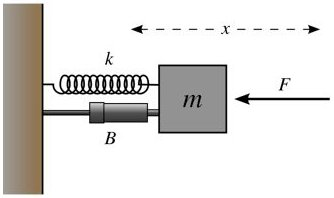
\includegraphics[width=0.5\textwidth]{figures/6_spring_model.jpg}
\footnote{\bkorel{cite wikipedia?}}
\end{figure}

\begin{figure}[!h]
\centering
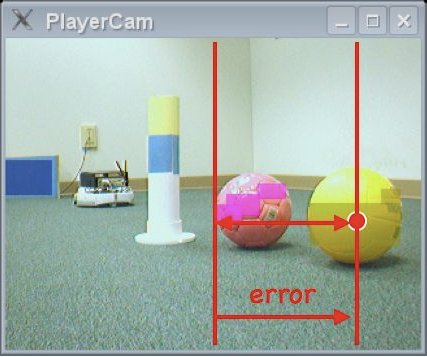
\includegraphics[width=0.5\textwidth]{figures/6_p_error.jpg}
\end{figure}

\end{itemize}

\section{Project Infrastructure}

\subsection{Player: Color Calibration / CMVision}

For color blobfinding, Player uses the \href{http://www.cs.cmu.edu/~jbruce/cmvision/}{CMVision} library to perform color segmentation and 
find relatively solid colored regions (or ``blobs''), as illustrated in Figure 2.  Specifically, Player has a ``cmvision'' device that uses 
data that is exposed to the client via the ``blobfinder'' proxy.  The cmvision device processes images provided by a camera device (such as 
``camera1394'') through Player's ``camera'' proxy.  The following is a snippet from a Player configuration file (extension ``.cfg'', loaded 
when a Player server is started) reflecting this description:

\begin{verbatim}
driver
(
  name "cmvision"
  provides ["blobfinder:0"]
  requires ["camera:0"]
  colorfile "blobcolors.txt"
)

driver
(
  name "camera1394"
  provides ["camera:0"]
)
\end{verbatim}

\begin{figure}[!b]
\centering
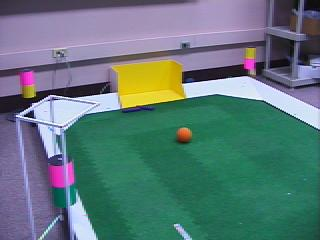
\includegraphics[width=.49\textwidth]{figures/6_video.jpg}
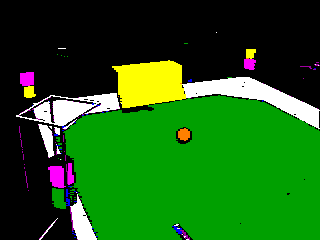
\includegraphics[width=.49\textwidth]{figures/6_classified.png}
\caption{An example of CMVision performing color segmentation on a robot soccer field (from the CMVision website).}
\label{fig:CMVision}
\end{figure}


The blobfinder specifically provides a bounding box around each image region containg a specified color of interest.  To perform blobfinding, 
Player's cmvision device requires knowledge of these colors of interest through a color calibration file, or ``colorfile'' (``blobcolors.txt'' 
in the example above). The colorfile contains two sections, listing each blob color in sequential order: 

\begin{itemize}
\item a ``[Colors]'' section specifying identifiers, as strings and integer triplets, for each blob color
\item a ``[Thresholds]'' section containing color thresholds (in YUV space) associated with each blob color
\end{itemize}

The following example ``blobcolors.txt'' illustrates the format of the colorfile:

\begin{verbatim}
[Colors]
(255,  0,  0) 0.000000 10 Red
(  0,255,  0) 0.000000 10 Green
(  0,  0,255) 0.000000 10 Blue

[Thresholds]
( 25:164, 80:120,150:240)
( 20:220, 50:120, 40:115)
( 15:190,145:255, 40:120)
\end{verbatim}

In this colorfile, the color ``Red'' has the integer identifier ``(255,0,0)'' or, in hexidecimal, 0x00FF0000 and YUV thresholds 
(25:164,80:120,150:240).  These thresholds are specified as a range.  Specifically, any pixel with YUV values within this range will be 
labelled with as the given blob color. Note: that YUV and RGB color coordinates are vastly different representations, you can refer to 
\href{http://en.wikipedia.org/wiki/YUV}{the Wikipedia YUV entry} and the Appendix for details.  

\begin{figure}[!t]
\centering
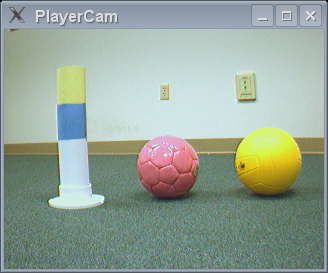
\includegraphics[width=.32\textwidth]{figures/6_objects.png}
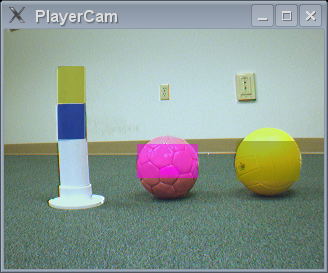
\includegraphics[width=.32\textwidth]{figures/6_blobs.png}
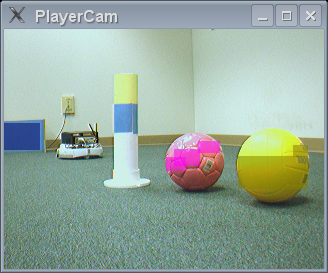
\includegraphics[width=.32\textwidth]{figures/6_blobs2.png}
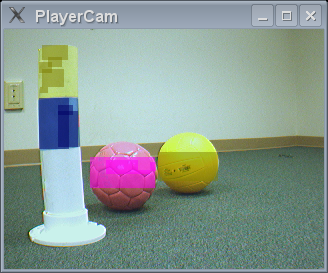
\includegraphics[width=.32\textwidth]{figures/6_blobs3.png}
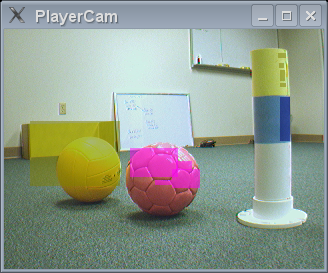
\includegraphics[width=.32\textwidth]{figures/6_blobs4.png}
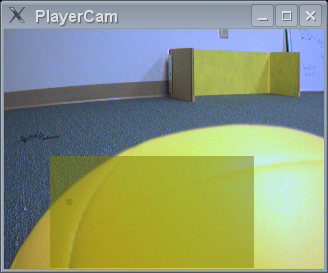
\includegraphics[width=.32\textwidth]{figures/6_blobs6.png}
\caption{An example of using playercam to color calibrate and perform blobfinding.  (Top left) 3 objects are placed in the robot's field 
of view and playercam is used to extract YUV values and thresholds for each object color.  (Other 5 images) Results from blobfinding with 
the resulting color calibration file from different robot locations and pushing the yellow ball.}
\label{fig:playercam}
\end{figure}


To calibrate the blobfinder, you will need to add appropriate lines in your colorfile containing identifiers and YUV thresholds.  Once you 
have an appropriately calibrated colorfile, the Player blobfinder will be able to detect color blobs, both in real and simulated 
environments, as illustrated above.  We have provided in playercam the ability to output YUV values associated with a pixel currently 
being displayed.  Clicking on a pixel in playercam will output to the terminal the associated XY location, RGB color values and YUV color 
values in the following format\footnote{The binary in {\it /course/cs148/bin/playercam\_yuv} is the one on system that provides proper YUV 
values}:

\begin{verbatim}
[51, 145] = RGB [0 140 0] : : YUV [82 81 69]
\end{verbatim}

Given this function in playercam, you can calibrate for the color of specific objects by sampling their pixel colors in playercam.  Start 
playercam and put objects of interest in the robot's view.  Click on a set of pixels for a single object that adequately describe the 
object's color.  Note: you may not want to click on all pixels of an object due to shadowing and specular (``shiny'') artifacts.  From 
these clicks, playercam will produce a list of YUV values.  Examine this list to find appropriate minimum and maximum values for each range.  
Note: if clicked pixels are chosen carefully, the straightforward min and max in each range can be used.  Otherwise, you may want to use 
some judgment in eliminating noisy outliers.  

Once you have a calibrated colorfile, you can restart the Player server and playercam to check the effectiveness of the new thresholds.  
playercam automatically overlays extracted blobs from the blobfinder using the colorfile in the configuration file. You can use the playerjoy 
or playerv utilities to then move the robot around the room and perform blobfinding of the objects from different viewpoints.  You may find 
small changes in camera perspective vastly change the performance of the blobfinder in such cases, you can sample pixel color values from 
these perspectives and adjust your YUV thresholds.  Also, make sure to properly order the [Colors] and [Thresholds] sections such that the 
blob color entries are aligned.  

{\bf Disclaimer}: The calibration process is not always easy and may take several iterations to get a working calibration.  Remember, 
the real world can be particular and unforgiving.  Small variations make a huge difference. So, be consistent and thorough.

\subsection{ROS: OpenCV?}

\section{Instructions}

The tasks for this assignment are as follows.

\begin{enumerate}
\item Generate a color calibration file for the blobfinder to recognize a solid yello colored ball and multi-colored fiducials.
\item Write a controller to seek out, find, and drive towards a single object. 
\item Extend this controller to continually drive between a set of objects in a sequential order.
\end{enumerate}


\subsection{Object Recognition and Seeking}

In this assignment, your Player client will need to distinguish three different Roomba Lab objects with the following integer order 
identifiers\footnote{Note, these do not necessarily need to be identifiers in the colorfile}:

\begin{enumerate}
\item Yellow ball 
\item Green over orange fiducial 
\item Orange over green fiducial 
\item Pink fiducial
\end{enumerate}

Given appropriate color calibration, recognizing single solid color objects should be straightforward.  However, fiducials used in 
robot soccer to indicate specific locations on the field may have multiple solid colors.  For example, the playercam image in Figure 3
has two solid colors stacked in a vertical order with similar shape dimensions.  In such cases, your Player 
client will need to specifically include perception routines to process the output of the blobfinder for multicolor fiducials.

Given a specific ordering (via file or command line), your client should drive the robot to visit each of the given Roomba Lab objects 
continuously in this order.  For example, the given ordering [3 1 2 4] should direct the robot to visit the green/orange fiducial, 
orange/green fiducial, yellow ball, pink fiducial, green/orange fiducial, etc.  A finite state machine is a good choice for controlling 
this decision making.  A proportional-derivative feedback controller with a form of wandering is a good choice for motion control.

\subsection{Teleoperation using playerv}

In playerv, the position and bumper proxies from Assignment 1 are still available, but we have also added a blobfinder proxy.  
Subscribe to the position and blobfinder proxies.  The blobfinder proxy should open up a window within playerv displaying the currently 
detected blobs and their bounding boxes.  You may also use the ``playercam'' application to see the camera images directly, and use 
playerjoy to control the robot.  

After selecting the ``command'' option for the position proxy, manually navigate the robot (using only the blobfinder for sensing) to 
the fiducial and ball using playerv.  Click and drag the rectangle in the middle of the window to drive the robot.  Keep trying manual 
navigation until you can successfully navigate between the red and blue fiducials using only the blobfinder.

\section{Expected Outcomes and Reports}

The following outlines our grading criteria:

\vspace{1cm}
\begin{tabular}{|l|l||l|l|}
\hline
{\large \bf Project Implementation} & \\
\hline
\hline
Color calibration & 20\% \\
$\rightarrow$ Is your color calibration file suitable for finding objects in the Roomba Lab? & \\
$\rightarrow$ What are the restrictions (camera pose, lighting, etc.) on your color blobfinding? & \\
\hline
Seeking a single object & 15\% \\
$\rightarrow$ Does your robot find, center, drive to non-occluded objects? & \\
$\rightarrow$ How close does your robot get to sought objects? & \\
\hline
Transitioning between objects & 8\% \\
$\rightarrow$ Does your robot properly switch to other objects after visiting an object? & \\
\hline
Controller Robustness & 7\% \\
$\rightarrow$ Does your controller run without interruption? & \\
\hline
\end{tabular}

\newpage
